\section{Le test du vide}
Au niveau du test du vide, le plus simple à mettre en oeuvre est un algorithme qui va tester chaque mot jusqu'à en trouver un qui est accepté. Ce fut donc la première étape. Cependant un algorithme pareil peut tourner indéfiniment si nous ne lui donnons pas de condition d'arrêt. Au niveau des conditions d'arrêt, nous pouvons lui fournir plusieurs choses, une limite d'itération de l'algorithme, une limite en taille de mot, une limite en nombre de noeuds parcourus, une limite sur le nombre de fois qu'on parcourt un même noeud,... Il y a beaucoup de possibilités à ce niveau.\par


\subsection{Taille des mots}
La première limite introduite fut sur la taille des mots, en effet, comme précédemment cité, Oscar H. Ibarra a introduit une limite sur la taille des mots pour ce type d'automate (avant d'être certain d'avoir un état acceptant ou un boucle dans l'automate). Cette limite prend en compte plusieurs caractéristiques de l'automate étudié: le nombre de compteur(s) '$m$', le nombre de lien(s) '$s$' et une constance '$c$':
\[ ( m \  s ) ^{s  c} \]
Cette version du test du vide a une complexité dans le pire des cas en $O(a!^{n})$ avec n, la taille maximale d'un mot, et a, le nombre de lettres dans l'alphabet de l'automate.\par
De manière plus générale, ce n'est pas réellement la taille du mot d'entrée qui est limitée mais le nombre de transitions possibles avant d'être certain d'avoir atteint un état acceptant ou d'être coincé dans une boucle. Dans un simple automate sans transition $\varepsilon$ (transition qui a pour seul but d'incrémenter ou décrémenter un et un seul compteur), c'est donc la taille du mot qui est limitée.\par

\subsection{Parcours en profondeur}
C'est la première version du test du vide développée. Un parcours en profondeur signifie qu'on travaille avec un stack (tas). On commence par mettre un mot vide dans le stack, ensuite on fait trouner une boucle qui va sortir le premier élément du stack (mot vide), on ajoute à ce mot une lettre de l'alphabet, on regarde si le mot est accepté puis on met le mot sur le stack (à faire pour chaque lettre), etc.. Pour un alphabet {A, B} et des mots de 4 lettres, cela ressemble à: A, AA, AAA, AAAA, AAAB, AABA, AABB, ABAA, etc..\par
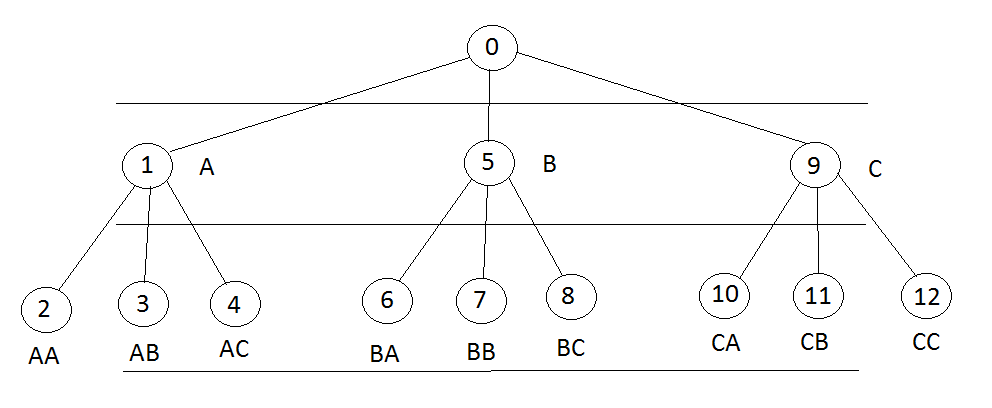
\includegraphics[height=3.5cm]{a5.png}
Bien sûr ceci est la représentation de l'ordre des mots, l'image ne représente en rien l'avancée dans le graphe.\par

\subsection{Parcours en largeur}
Dans cette version, nous utilisons un heap (pile). C'est le même algorithme en remplaçant le stack par un heap, le premier rentré sera donc le premier servi, un parcours va ressembler à: A, B, AA, AB, BA, BB, AAA, AAB, ABA, ABB, etc..\par
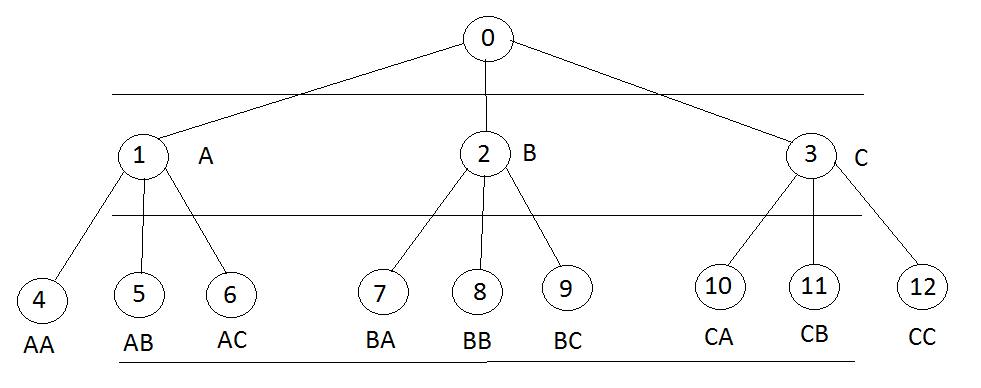
\includegraphics[height=3.4cm]{a4.png}
Bien sûr ceci est la représentation de l'ordre des mots, l'image ne représente en rien l'avancée dans le graphe.\par

\subsection{Parcours en profondeur dynamique}
Dans le simple parcours en profondeur, on testait mot par mot, ce qui signifie parcourir le graphe pour AAA (2 transitions d'états) et pour AAAA (3 transitions d'états), des étapes sont ici répétées. En effet, deux transitions sont identiques.\par
On peut alors améliorer l'algorithme en regardant lettre par lettre, c'est le parcours dynamique. Nous regardons les mots dans le même ordre que le simple parcours en profondeur mais sans les répétitions de transition. Pour tenter d'être plus clair, voici un exemple d'étapes:\par
Pour un automate d'alphabet \{A,B,C\} qui n'accepte que les mots avec un C en $3^{eme}$ position. Cet automate boucle sur le premier état et incrémente un compteur pour chaque lettre, si le compteur est égal à 2 et la lettre suivante est un C, on passe à l'état 2, état acceptant.
\begin{enumerate}
    \item compteur = 0, état 1  (initialisation)
    \item A -> compteur = 1, état 1 (mot testé == A)
    \item A -> compteur = 2, état 1 (mot testé == AA)
    \item A -> compteur = 3, état 1 (mot testé == AAA)
    \item A -> compteur = 4, état 1 (mot testé == AAAA)
    \item taille maximale d'un mot => on fait un pas en arrière et continue avec la lettre suivante
    \item B -> compteur = 4, état 1 (AAAB)
    \item taille maximale d'un mot => on fait un pas en arrière et continue avec la lettre suivante
    \item C -> compteur = 4, état 1 (AAAC)
    \item taille maximale d'un mot => on fait un pas en arrière et continue avec la lettre suivante
    \item B -> compteur = 3, état 1 (AAB)
    \item ... les 3 lettres en dernière position ... retour en arrière ...
    \item C -> compteur = 2, état 2 (AAC)
    \item le mot est accepté donc l'algorithme s'arrête, l'automate accepte au moins un mot.
\end{enumerate}\par
Grâce à cette amélioration nous réduisons la complexité dans le pire des cas à  $O(a^{n})$ \par

\subsection{Parcours en profondeur dynamique avec sauvegardes d'états}
On rajoute encore une couche supplémentaire, nous allons maintenant nous souvenir d'états dans l'algorithme. Une sauvegarde d'état est un 2-tuple composé de l'état $q_{i}$ dans lequel nous sommes ainsi que la liste C des i compteurs  $c_{i}$.
\[ save = (q_{i}, C) \]
Pour chaque sauvegarde, nous allons ajouter les différentes lettres au mot puis garder cette sauvegarde dans un vecteur. Si cette sauvegarde est déjà présente dans le vecteur, nous sommes déjà passés par ce même état avec les mêmes valeurs de compteurs, nous sommes soit dans une boucle soit, simplement, dans deux parcours identiques. Si tel est le cas, nous arrêtons de parcourir le graphe dans cette direction.\par
En résumé, nous évitons des répétitions et surtout de nous prendre dans des boucles interminables.\par
Cette amélioration va augmenter la complexité dans le pire des cas à  $O(a^{2n})$, en effet pour chaque état rencontré, nous devons regarder si il a déjà été parcouru. \textbf{Cependant}, nous allons réduire la complexité moyenne pour des automates complexes. En effet, ces automates sont destinés à contenir des boucles.\par

\subsection{Parcours depuis un état acceptant:}
Il est possible de partir d'un état acceptant et de voir si on arrive à retourner à l'état initial. Le but étant d'éviter que notre parcours s'écarte de la solution pour n'y revenir qu'à la fin (pire des cas d'un parcours entier depuis un état initial).\par
Cependant cela requiert d'inverser notre graphe, donc inverser l'ordre des noeuds et le sens des liens ainsi qu'un update au niveau des comparaisons lorsqu'un lien compare un compteur ET incrémente/décrémente le même compteur.\par
En addition de cette inversion, il faut compléter le graphe inversé au niveau du nouvel état initial avec des transitions $\varepsilon$ pour avoir les valeurs acceptantes de compteur.\par
Il est encore possible de pousser plus loin, dans le cas d'un automate avec plusieurs états acceptants, nous pouvons créer un nouvel état acceptant ainsi que des liens transitions $\varepsilon$ en bouclant sur ce dernier. On peut dès lors ajouter des liens vers les anciens états acceptants avec des comparaisons sur les compteurs pour avoir leurs valeurs acceptantes.\par
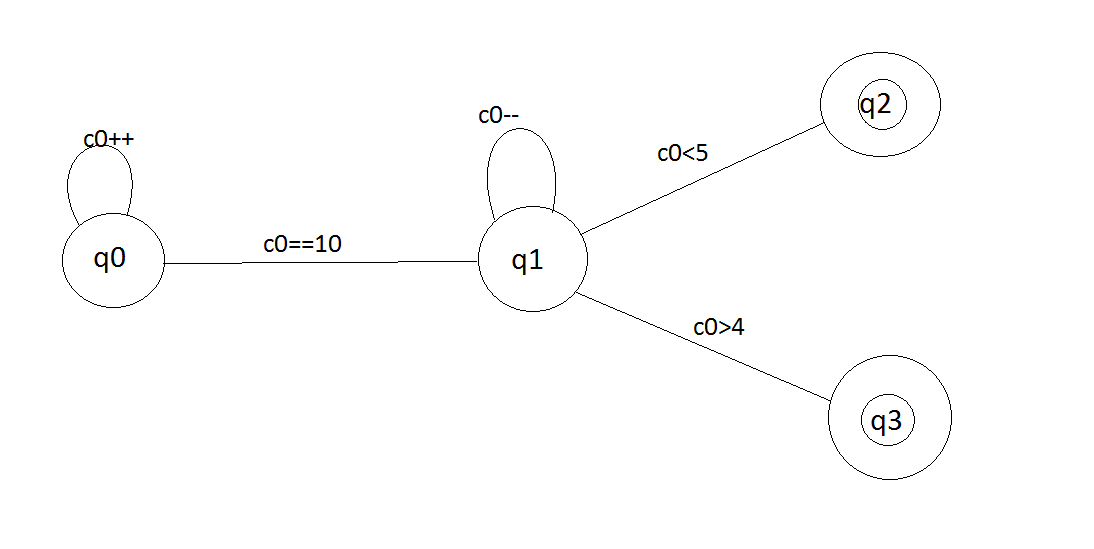
\includegraphics[height=4cm]{a0.png}
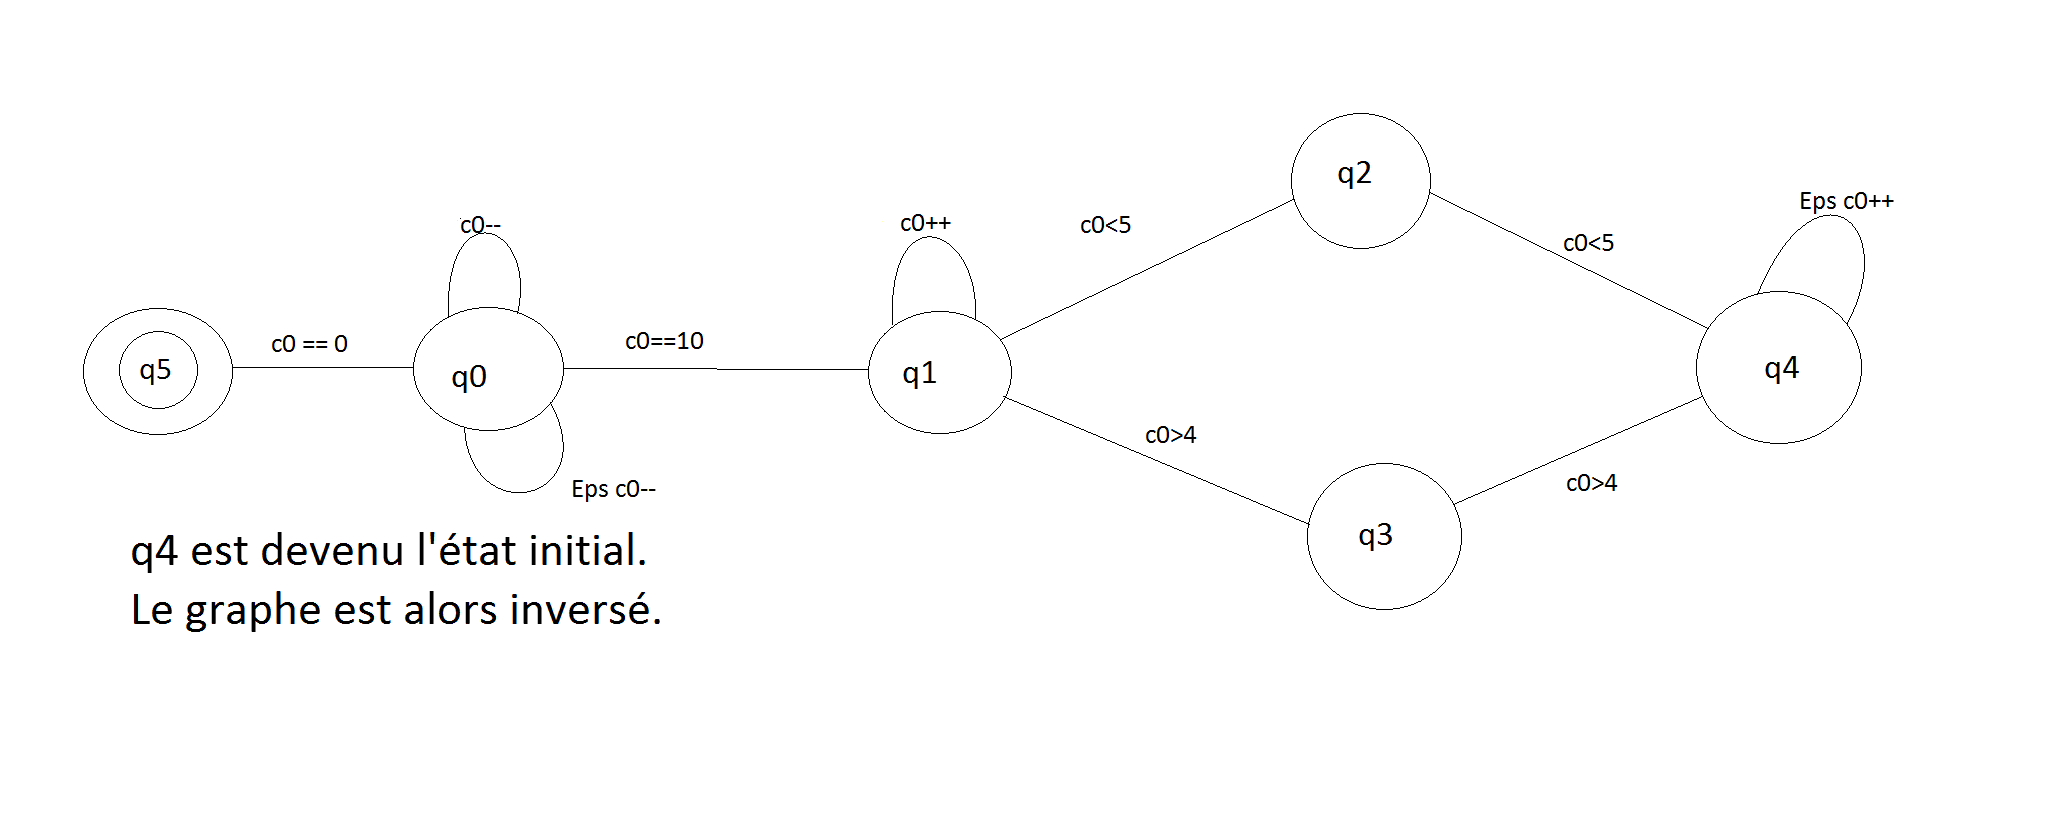
\includegraphics[height=3.5cm]{a1.png}
\par
Toutes les précédentes versions peuvent être utilisées avec un graphe inversé\par



\subsection{Améliorations possibles}
Voici des améliorations qui n'ont pas été implémentées.

\subsubsection{Parcours dans les deux sens:}
Il est possible de réaliser un parcours qui part dans les deux sens et tente de trouver un même état avec les mêmes valeurs de compteur. \par
Pourquoi est ce que ce serait une amélioration? Il faut s'imaginer un parcours comme un triangle, plus on avance dedans, plus on a de chance de s'écarter de l'état initial (pas forcément, vu que c'est un graphe, tout est possible) ou des valeurs de compteurs initiales.\par
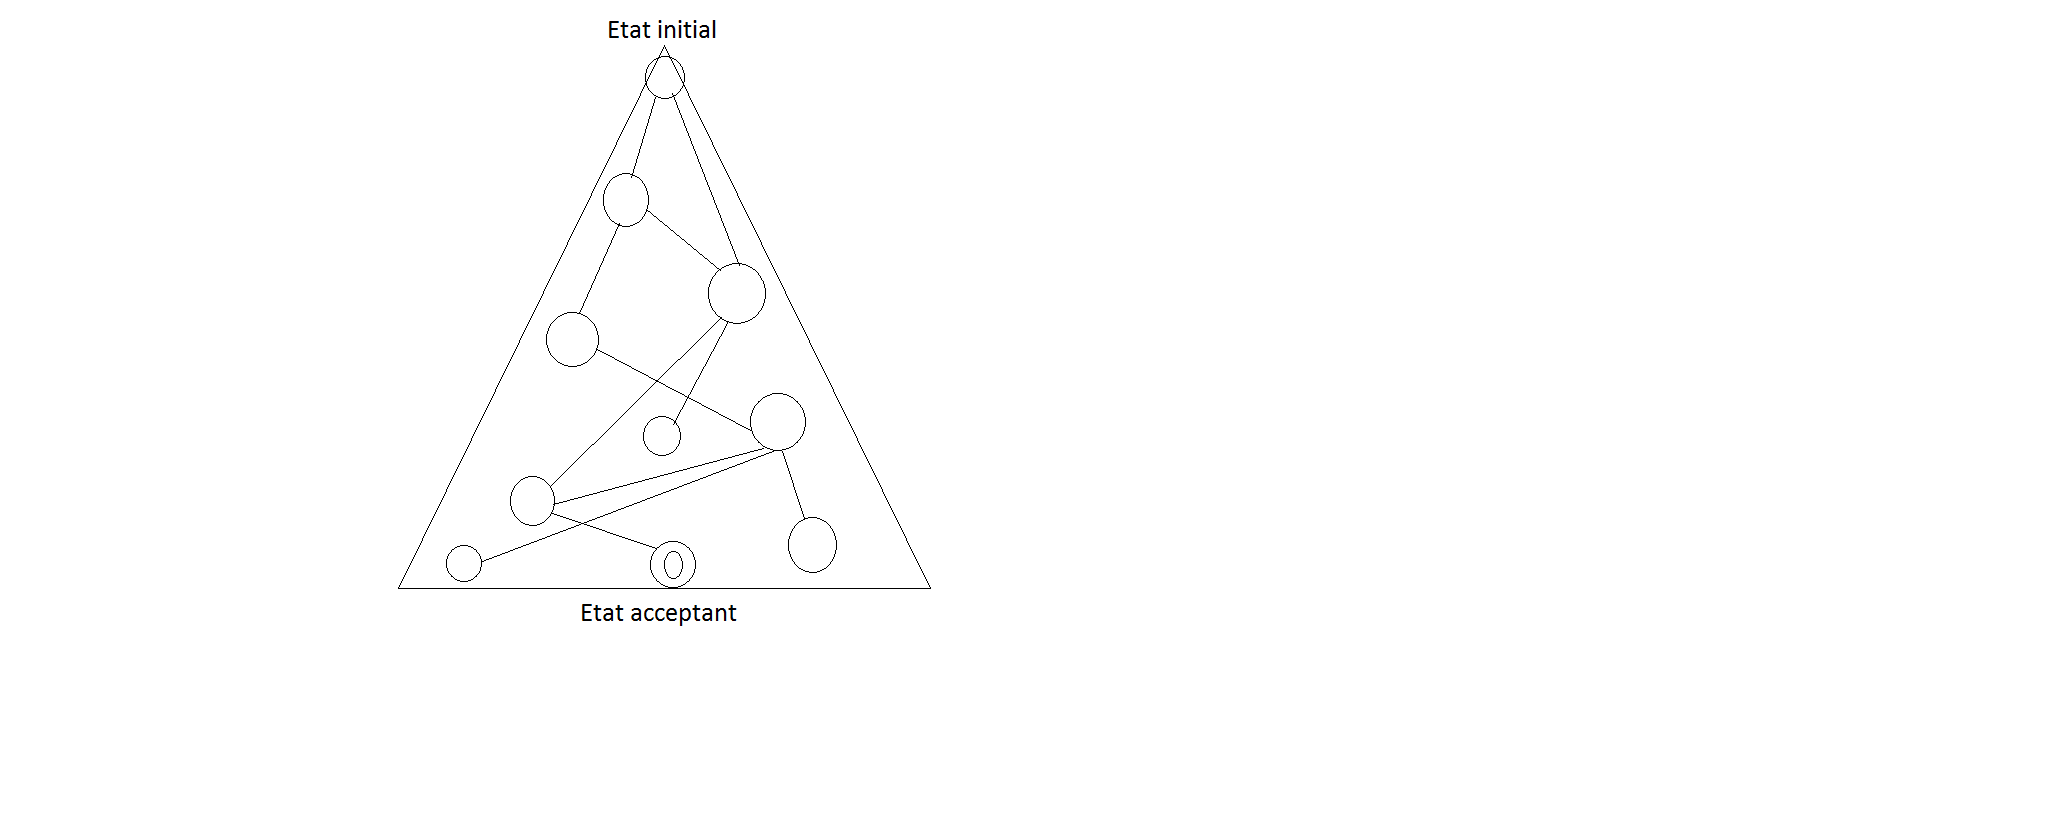
\includegraphics[height=5cm]{a2.png}
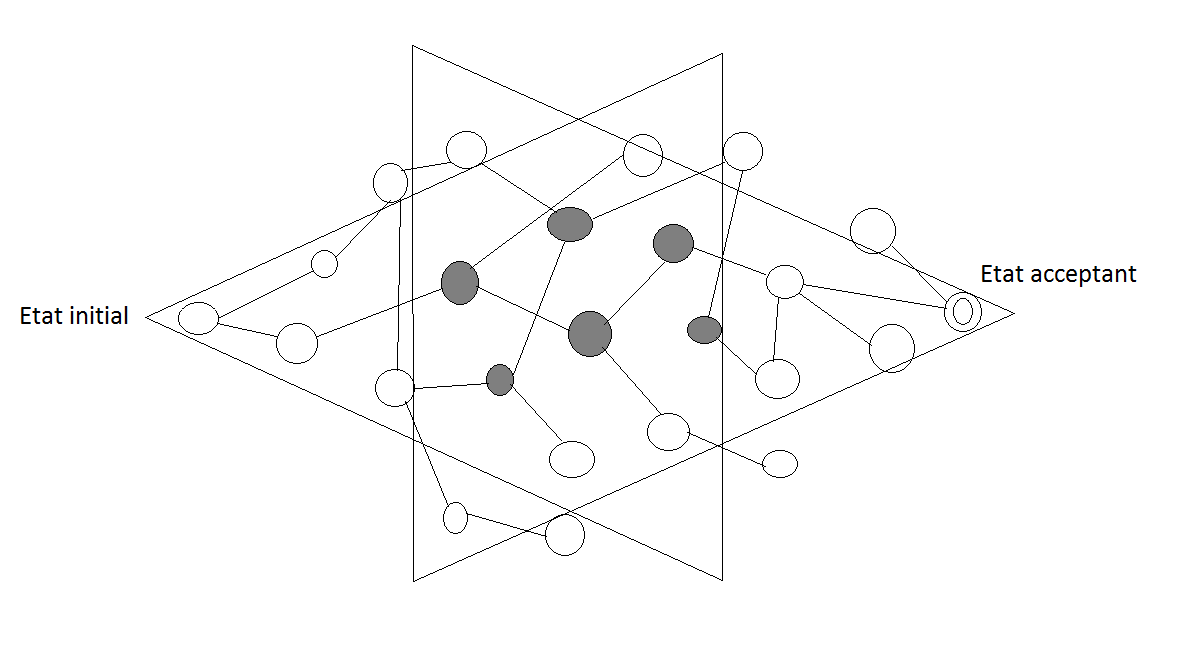
\includegraphics[height=5cm]{a3.png}\par
Nous visons dés lors ces noeuds surlignés en gris, en tentant d'éviter de s'aventurer dans les noeuds qui peuvent nous mener loin de l'état acceptant. Il faudrait obligatoirement utiliser un parcours en largeur pour ce type d'amélioration.\par

\subsubsection{Tout en un:}
Nous pourrions aussi tester un algorithme qui en combine plusieurs (par exemple un algorithme qui parcourt en profondeur et en largeur en même temps) et, ce, dans le but d'en tirer les bénéfices des deux.\par
Mais comme dit précédemment, chaque automate est fort différent et un algorithme en profondeur peut être instantané dans le meilleur des cas ou extrêmement long dans le pire des cas. Imaginons que le seul mot accepté soit un mot rempli de la dernière lettre de l'alphabet.
